\section{本文工作}

%%%%%%%%%%%%%%%%%%%%%%%%%%%%%%%%%%%%%%%%	
\subsection{概述}

%%%%%%%%%%%%%%%
\begin{frame}{工作概述}
  \begin{table}[]
	\centering
	\caption{本文落实\idea{}研究理念.}
	\renewcommand\arraystretch{1.6}
	\resizebox{\textwidth}{!}{%
	  \begin{tabular}{cc|c|c|c|c|}
		\cline{3-6}
		\multicolumn{2}{c|}{} & \multicolumn{2}{c|}{\textbf{读写寄存器}} & \multicolumn{2}{c|}{\textbf{事务}} \\ \cline{3-6} 
		\multicolumn{2}{c|}{} & 多处理器系统 & \cellcolor{red!80}{分布式系统} & \textcolor{gray}{多处理器系统} & \cellcolor{red!80}{分布式系统} \\ \hline

		\multicolumn{2}{|c|}{\textbf{\ideadt{}}} & {\begin{tabular}[c]{@{}c@{}}{\small 相关工作丰富}\\ {\small 理论扎实}\end{tabular}}
		& \begin{tabular}[c]{@{}c@{}}{\small 渐成趋势}\\ {\small 理论欠缺}\end{tabular} 
		& \multirow{2}{*}[-3em]{\begin{tabular}[c]{@{}c@{}}\textcolor{gray}{\small 软件}\\ \textcolor{gray}{\small 事务内存}\end{tabular}}
		& \cellcolor{brown!80}{\begin{tabular}[c]{@{}c@{}}{\small 探索阶段}\\ {(RVSI)}\end{tabular}} \\ \cline{1-4} \cline{6-6}

		\multicolumn{1}{|c|}{\multirow{2}{*}[-1em]{\textbf{\idearm{}}}} & 验证 
		& \begin{tabular}[c]{@{}c@{}}{\small 典型模型}\\ {\small 理论全面}\end{tabular} 
		& \cellcolor{brown!80}{\begin{tabular}[c]{@{}c@{}}{\small 弱模型验证}\\ {(VPC)}\end{tabular}}
		& 
		& \begin{tabular}[c]{@{}c@{}}{\small 理论全面}\\ {\small 指导协议设计}\end{tabular}
		\\ \cline{2-4} \cline{6-6} \hhline{*{3}{~}-*{2}{~}}

		\multicolumn{1}{|c|}{} & 量化 
		& \begin{tabular}[c]{@{}c@{}}{\small 暂无}\\ {\small 强调正确性}\end{tabular}
		& \cellcolor{brown!80}{\begin{tabular}[c]{@{}c@{}}{\small 量化协议}\\ {(PA2AM)}\end{tabular}}
		&  
		& \begin{tabular}[c]{@{}c@{}}{\small 量化协议难}\\ {\small 相关工作少}\end{tabular} 
		\\ \hline
	  \end{tabular}
	}
  \end{table}
\end{frame}
%%%%%%%%%%%%%%%
%%%%%%%%%%%%%%%%%%%%%%%%%%%%%%%%%%%%%%%%
\subsection{VPC: Pipelined-RAM 一致性验证}

\newcommand{\pram}{Pipelined-RAM}
\newcommand{\PRAM}{PRAM}
\newcommand{\vpc}[1]{\ifthenelse{\isempty{#1}{}}{\textsf{VPC}}{\textsf{VPC-\MakeUppercase{#1}}}} 
\newcommand{\npc}{$\sf{NP}$-complete}
\newcommand{\npcn}{$\sf{NP}$-completeness}
\newcommand{\rwclosure}{\textsc{RW-Closure}}
\newcommand{\readcentric}{\textsc{Read-Centric}}
%%%%%%%%%%%%%%%
\begin{frame}{VPC 工作在技术框架中的位置}
  \fig{width = 0.50\textwidth}{figures/3d-framework-vpc.pdf}{VPC --- \pram{} {\small (\PRAM{})} 一致性验证.}
\end{frame}
%%%%%%%%%%%%%%%
\begin{frame}{研究动机}
  \question{问题: 为什么要验证 \PRAM{} 一致性?}
  \vspace{0.10cm}

  \begin{description}
    \setlength{\itemsep}{10pt}
	\item[验证:] 用户与商家就数据一致性签订 SLA {\small (Service Level Agreement)} 协议
	  \citeinbeamer{Amazon}{SOSP}{07} \citeinbeamer{Golab}{PODC}{11}
	  \vspace{2pt}
	  \begin{itemize}
		\item \textcolor{teal}{[商家]} 系统测试手段之一
		\item \textcolor{teal}{[用户]} 确认系统是否提供了其所声称的数据一致性 
	  \end{itemize}
	\pause
	\item[PRAM:] 存储系统常提供``会话'' {\small (session)} 一致性\\
      \citeinbeamer{Saito}{CSUR}{05} \citeinbeamer{Terry}{CACM}{13}
	  \vspace{2pt}
      \begin{itemize}
		\item 包含了弱一致性的诸多变体 
		\item 近似于 PRAM 一致性 \citeinbeamer{Brzezi$\acute{\text{n}}$ski}{PDP}{04} \citeinbeamer{Bailis}{VLDB}{13}
      \end{itemize}
  \end{description}
\end{frame}
%%%%%%%%%%%%%%%
\begin{frame}{VPC 问题定义}
  \begin{cdef}[VPC: Verifying PRAM Consistency]
    VPC 判定问题:
	\vspace{8pt}
    \begin{description}
	  \setlength{\itemsep}{8pt}
      \item[实例:] 系统执行 {\small (execution $e$)}
      \item[问题:] 该执行 $e$ 是否满足 PRAM 一致性模型 {\small ($\mathcal{C}$)}? 
		\[
		  e \in \mathcal{C} \Rightarrow \set{0,1}?
		\]
    \end{description}    
  \end{cdef}
\end{frame}
%%%%%%%%%%%%%%%
\begin{frame}{VPC 问题定义}
  \begin{cdef}[系统执行]
	系统执行 ($e$) $\triangleq$ $\{h_p \mid h_p: \text{进程 } \;p \text{ 上的读写操作序列}\}$

	\vspace{0.30cm}
	\textcolor{blue}{规模 $n$:} 系统执行中操作的总数
  \end{cdef}

  \fignocaption{width = 0.50\textwidth}{figures/execution-example.pdf}
\end{frame}
%%%%%%%%%%%%%%%
\begin{frame}{VPC 问题定义}
  \begin{cdef}[\PRAM{} 一致性模型]
	\begin{center}
	  系统执行 $e$ 满足 \PRAM{} 一致性 \\
	  $\iff$\\
	  $\forall p:$ $p$ 上\textcolor{blue}{所有操作}与其它进程上所有\textcolor{blue}{写操作}存在\textcolor{red}{合法}调度.
	\end{center}
  \end{cdef}

  \fignocaption{width = 0.50\textwidth}{figures/execution-example.pdf}

  \pause
  \vspace{-0.80cm}

  \begin{gather*}
	p_{0}: Wf2\; Wf1\; Wz2\; Wz1\; Wy2\; Wy1\; \textcolor{brown}{Rf1} 
	Wx5\; Wx3\; Wx2\; Wc1\; \textcolor{brown}{Rc1} \\
	\textcolor{brown}{Rz1} \textcolor{brown}{Ry1}
	Wa1\; \textcolor{brown}{Ra1} Wb1\; \textcolor{brown}{Rb1} \textcolor{brown}{Rx2}
  \end{gather*}
\end{frame}
%%%%%%%%%%%%%%%
\begin{frame}{VPC 问题分类}
  \begin{table}[!t]
    \centering
	\caption{VPC 问题的四种变体 (按``执行''的类型) 及复杂度分析 ($\textcolor{red}{[\ast]}$\textcolor{red}{: 本文工作}).}
	\renewcommand\arraystretch{1.2}
    \begin{tabular}{|c|c|c|}
      \hline
      & \it (S)ingle variable  & \it (M)ultiple variables
      \\ \hline
	  {\it write (D)uplicate values} &
	  \innercell{c}{VPC-SD \\ \uncover<2->{\textcolor{red}{\small (\npc{}) $[\ast]$}}} &
	  \innercell{c}{VPC-MD \\ \uncover<2->{\textcolor{red}{\small (\npc{}) $[\ast]$}}}
      \\ \hline
	  \only<1-2>{\it write (U)nique value}\only<3>{\cellcolor{brown!80}{\it write (U)nique value}} &
	  \innercell{c}{VPC-SU \\ \uncover<2->{\textcolor{blue}{\small (P) \citeinbeamer{Golab}{PODC}{11}}}} &
	  \innercell{c}{VPC-MU \\ \uncover<2->{\textcolor{red}{\small (P) $[\ast]$}}}
      \\ \hline
    \end{tabular}
  \end{table}

  \vspace{10pt}
  
  \uncover<3->{\textcolor{brown}{\centerline{Read-mapping \citeinbeamer{Gibbons}{SICOMP}{97}: $\forall r, \exists! w, f(r) = w$.}}}
\end{frame}
%%%%%%%%%%%%%%%
\begin{frame}{VPC-SD (VPC-MD) 是 \npc{} 问题}
  多项式规约: 从 \textsc{Unary 3-Partition} 到 \vpc{sd}.

  \fig{width = 0.40\textwidth}{figures/vpcsd-npc.pdf}{对应于 \textsc{Unary 3-Partition} 实例 $A = \{2,2,1,1,1,1\}, m = 2, B = 4$ 的 VPC 执行.} 
\end{frame}
%%%%%%%%%%%%%%%
\begin{frame}{VPC-MU 的多项式算法 \rwclosure{}}
  \begin{figure}[h!]
    \centering
    \begin{adjustbox}{max totalsize = {0.60\textwidth}{1.00\textheight}, center}
	  % http://tex.stackexchange.com/questions/54794/using-a-pgfplots-style-legend-in-a-plain-old-tikzpicture#54834

% argument #1: any options
\newenvironment{customlegend}[1][]{%
    \begingroup
    % inits/clears the lists (which might be populated from previous
    % axes):
    \csname pgfplots@init@cleared@structures\endcsname
    \pgfplotsset{#1}%
}{%
    % draws the legend:
    \csname pgfplots@createlegend\endcsname
    \endgroup
}%

% makes \addlegendimage available (typically only available within an
% axis environment):
\def\addlegendimage{\csname pgfplots@addlegendimage\endcsname}

%%--------------------------------

% definition to insert numbers
\pgfkeys{/pgfplots/number in legend/.style={%
        /pgfplots/legend image code/.code={%
            \node at (0.295,-0.0225){#1};
        },%
    },
}
%%%%%%%%%%%%% For Legend %%%%%%%%%%%%%%%%%%%%%%

\begin{tikzpicture}[read/.style = {fill = orange, font = \Large}, 
write/.style = {fill = lightgray, font = \Large},
on grid, every node/.style = {node distance = 1.0cm and 1.6cm}, 
po/.style = {->, very thick, blue}]
%   	      \draw[step = {(1.5,1)}, style=help lines] (-1.5,0) grid (10.5,4);
	% process 0
	\begin{scope}[yshift = 4.0cm]
		\node (wy1) [write] at (0,0) {$Wy1$};
		\node (rf1) [read, right = of wy1] {$Rf1$};
		\node (rc1) [read, right = of rf1] {$Rc1$};
		\node (rz1) [read, right = of rc1] {$Rz1$};
		\node (ry1) [read, right = of rz1] {$Ry1$};
		\node (ra1) [read, right = of ry1] {$Ra1$};
		\node (rb1) [read, right = of ra1] {$Rb1$};
		\node (rx2) [read, right = of rb1] {$Rx2$};
	\end{scope}

	% process 1
	\begin{scope}
		\node (wf1) [write, node distance = 1.5cm, below = of rf1] {$Wf1$};
		\node (wx2) [write, node distance = 1.5cm and 3.0cm, below left = of rx2] {$Wx2$};
		\node (wc1) [write, node distance = 3.0cm, right = of wx2] {$Wc1$};
	\end{scope}

	% process 2
	\begin{scope}[]
		\node (wa1) [write, node distance = 3.0cm and 3.5cm, below left = of ra1] {$Wa1$};
		\node (wx3) [write, left = of wa1] {$Wx3$};
		\node (wz2) [write, left = of wx3] {$Wz2$};
		\node (wf2) [write, left = of wz2] {$Wf2$};
	\end{scope}

	% process 3
	\begin{scope}[]
		\node (wb1) [write, node distance = 4.5cm and 0.5cm, below right = of rb1] {$Wb1$};
		\node (wx5) [write, left = of wb1] {$Wx5$};
		\node (wy2) [write, left = of wx5] {$Wy2$};
		\node (wz1) [write, left = of wy2] {$Wz1$};
	\end{scope}

\begin{scope}[dotted, very thick, every node/.style = {font = \Large}]
  \node (lvnode) [node distance = 1.5cm, left = of wy1] {};
  \node (rvnode) [node distance = 1.0cm, right = of rx2] {};
  
  \node (p0) at (lvnode) {$p_0$};
  \draw (p0) -- (wy1);
  \node (rp0) at (rvnode) {};
  \draw (rx2) -- (rp0);

  \node (p1) [node distance = 1.5cm, below = of p0] {$p_1$};
  \draw (p1) -- (wf1);
  \node (rp1) [node distance = 1.5cm, below = of rp0] {};
  \draw (wc1) -- (rp1);

  \node (p2) [node distance = 1.5cm, below = of p1] {$p_2$};
  \draw (p2) -- (wf2);
  \node (rp2) [node distance = 1.5cm, below = of rp1] {};
  \draw (wa1) -- (rp2);

  \node (p3) [node distance = 1.5cm, below = of p2] {$p_3$};
  \draw (p3) -- (wz1);
  \node (rp3) [node distance = 1.5cm, below = of rp2] {};
  \draw (wb1) -- (rp3);
\end{scope}

\uncover<2->{
    % program order
    \begin{scope}[]
	  \draw[po] (wy1) -- (rf1);
	  \draw[po] (rf1) -- (rc1);	  
	  \draw[po] (rc1) -- (rz1);
	  \draw[po] (rz1) -- (ry1);
	  \draw[po] (ry1) -- (ra1);
	  \draw[po] (ra1) -- (rb1);
	  \draw[po] (rb1) -- (rx2);

	  \draw[po] (wf1) -- (wx2);
	  \draw[po] (wx2) -- (wc1);

	  \draw[po] (wf2) -- (wz2);
	  \draw[po] (wz2) -- (wx3);
	  \draw[po] (wx3) -- (wa1);

	  \draw[po] (wz1) -- (wy2);
	  \draw[po] (wy2) -- (wx5);
	  \draw[po] (wx5) -- (wb1);
	\end{scope}
  }

  \uncover<3->{
	% read-write mapping
	\begin{scope}[rwmap/.style={->, violet, very thick}]
		\draw [rwmap] (wf1) -- (rf1);
		\draw [rwmap] (wc1) [out = 160, in = -15] to (rc1.south);
		\draw [rwmap] (wz1) -- (rz1);
% 		\draw [rwmap] (wy1) [out = 20, in = 160] to (ry1);
		\draw [rwmap] (wy1) [out = -23, in = -157] to (ry1);
		\draw [rwmap] (wa1.north) -- (ra1.south);
		\draw [rwmap] (wb1) -- (rb1);
		\draw [rwmap] (wx2) -- (rx2.south);
	\end{scope}
  }

	% wprimew edge 
	\begin{scope}[wprimew/.style = {->, purple, dashed, ultra thick}]
	  \uncover<4->{\draw[wprimew] (wx3.north) to node [font = \Large, near start, color = black] {1} (wx2);}
	  \uncover<5->{\draw[wprimew] (wx5) to node [font = \Large, color = black] {2} (wx2);}

	  \uncover<6->{\draw[wprimew] (wz2.south) to [out = -45, in = 180] node [font = \Large, color = black] {3} (wz1);}
	  \uncover<7->{\draw[wprimew] (wf2.north) to node [font = \Large, color = black] {5} (wf1.west);}
	  \uncover<8>{\draw[wprimew] (wy2.north) to [out = 100, in = -20] node [font = \Large, very near start, color = black] {4} (wy1.south);}
	\end{scope}

\coordinate (legend-pos) at ($0.5*(p0) + 0.5*(rx2)$);

\begin{customlegend}[legend columns = -1, 
legend entries = { % <= in the following there are the entries
	$\; $ program order,
    $\; $ write-to order,
    $\; $ $w'wr$ order
},
legend style = {at = {($(legend-pos) + (0,1)$)}, anchor = south, /tikz/every even column/.append style = {column sep=0.5cm}, font = \Large}] % <= to define position and font legend
% the following are the "images" and numbers in the legend
    \addlegendimage{->, very thick, blue}
    \addlegendimage{->, violet, very thick}
    \addlegendimage{->, purple, dashed, ultra thick}
\end{customlegend}

\end{tikzpicture}
    \end{adjustbox}
	\caption{\rwclosure{} 算法示例: 在传递闭包之上迭代应用 $w'wr$ 规则.}
  \end{figure}

  \uncover<4->{\fig{width = 0.25\textwidth}{figures/wprimewr-order.pdf}{$w'wr$ 规则.}}
\end{frame}
%%%%%%%%%%%%%%%
\begin{frame}{VPC-MU 的多项式算法 \rwclosure{}}
  \begin{ctheorem}[\rwclosure{} 算法正确性]
	\begin{center}
	  \vpc{mu} 实例满足 \PRAM{} 一致性\\
		$\iff$\\
	  \rwclosure{} 算法所得图是 DAG 图.
	\end{center}
  \end{ctheorem}

  \pause
  \vspace{0.80cm}

  \rwclosure{} 算法复杂度: 
  \[
    \underbrace{O(n^2)}_{\textrm{\#loops}} \quad\cdot
	\underbrace{O(n^3)}_{\textrm{transitive closure}}  = O(n^5)
  \]
\end{frame}
%%%%%%%%%%%%%%%
\begin{frame}{VPC-MU 的多项式算法 \readcentric{}}
  \rwclosure{} 算法的缺点:
  \begin{itemize}
	\item 在全图上应用 $w'wr$ 规则
	\item 应用 $w'wr$ 规则无特定顺序
  \end{itemize}

  \pause
  \vspace{0.50cm}

  \readcentric{} 算法要点:
  \begin{itemize}
	\item \textcolor{blue}{增量式}调度每个读操作
	\item 在读操作诱导的\textcolor{blue}{局部子图}上按\textcolor{blue}{逆拓扑序}应用 $w'wr$ 规则
  \end{itemize}

  \pause
  \vspace{0.60cm}
  \rwclosure{} 算法复杂度: 
  \[
    \underbrace{O(n)}_{\textrm{iterations}} \cdot
	\underbrace{O(n^3)}_{\textsc{Topo-Schedule}} = O(n^4)
  \]
\end{frame}
%%%%%%%%%%%%%%%
\begin{frame}{实验评估}
  实验目的:
  \begin{enumerate}
	\item 考察 \readcentric{} 算法的实际效率 
	  \textcolor{blue}{\small ({\it vs.} 渐近时间复杂度)}
	\item 对比 \readcentric{} 算法与 \rwclosure{} 算法的效率
  \end{enumerate}

  \pause
  \vspace{0.50cm}

  两类负载:
  \begin{enumerate}
	\item 随机生成的系统执行
	\item 满足 \PRAM{} 一致性的系统执行 \textcolor{red}{\small ($\approx$ 最坏情况输入)}
  \end{enumerate}
\end{frame}
%%%%%%%%%%%%%%%
\begin{frame}{实验评估}
  \begin{figure}[t]
	\centering
	\begin{subfigure}[t]{0.50\textwidth}
	  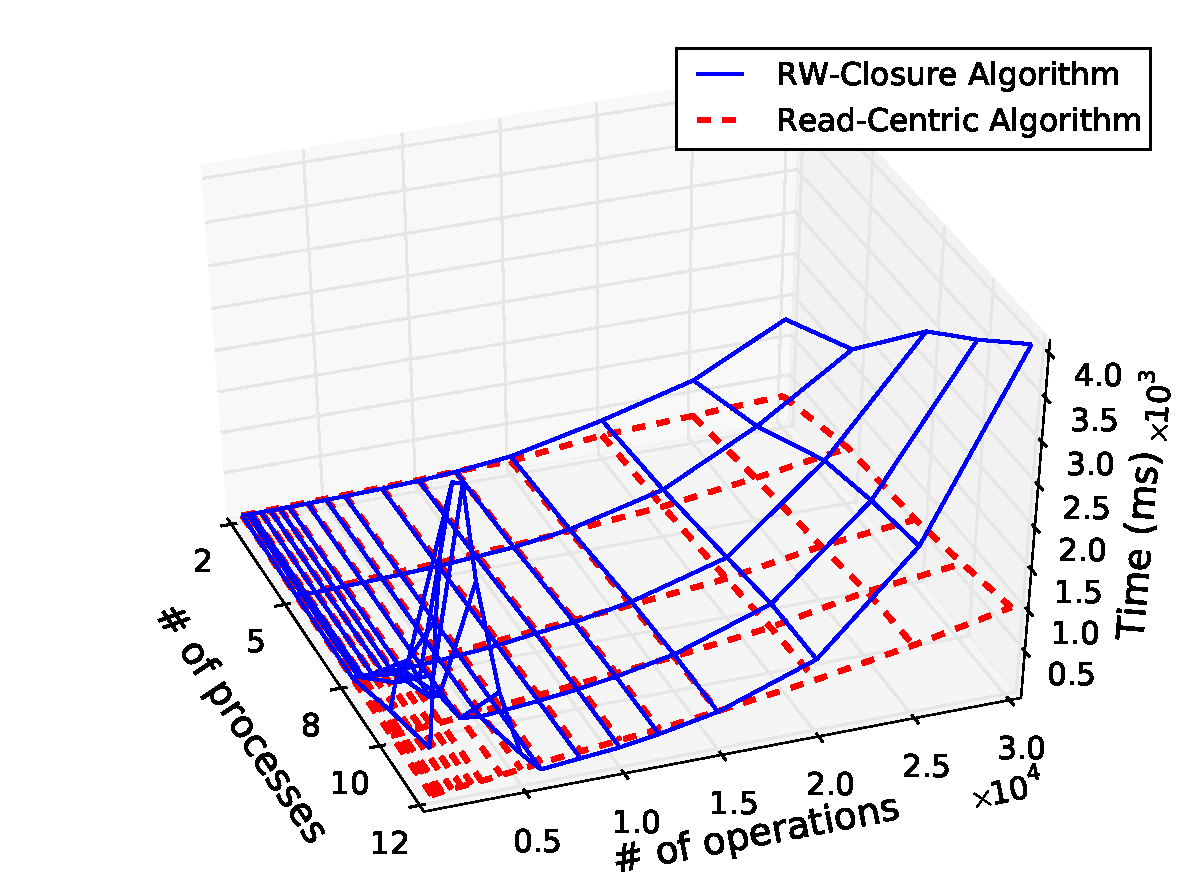
\includegraphics[width = 0.80\textwidth]{figures/vpc-random-cmp.pdf}
	\end{subfigure}%
	~
	\begin{subfigure}[t]{0.50\textwidth}
	  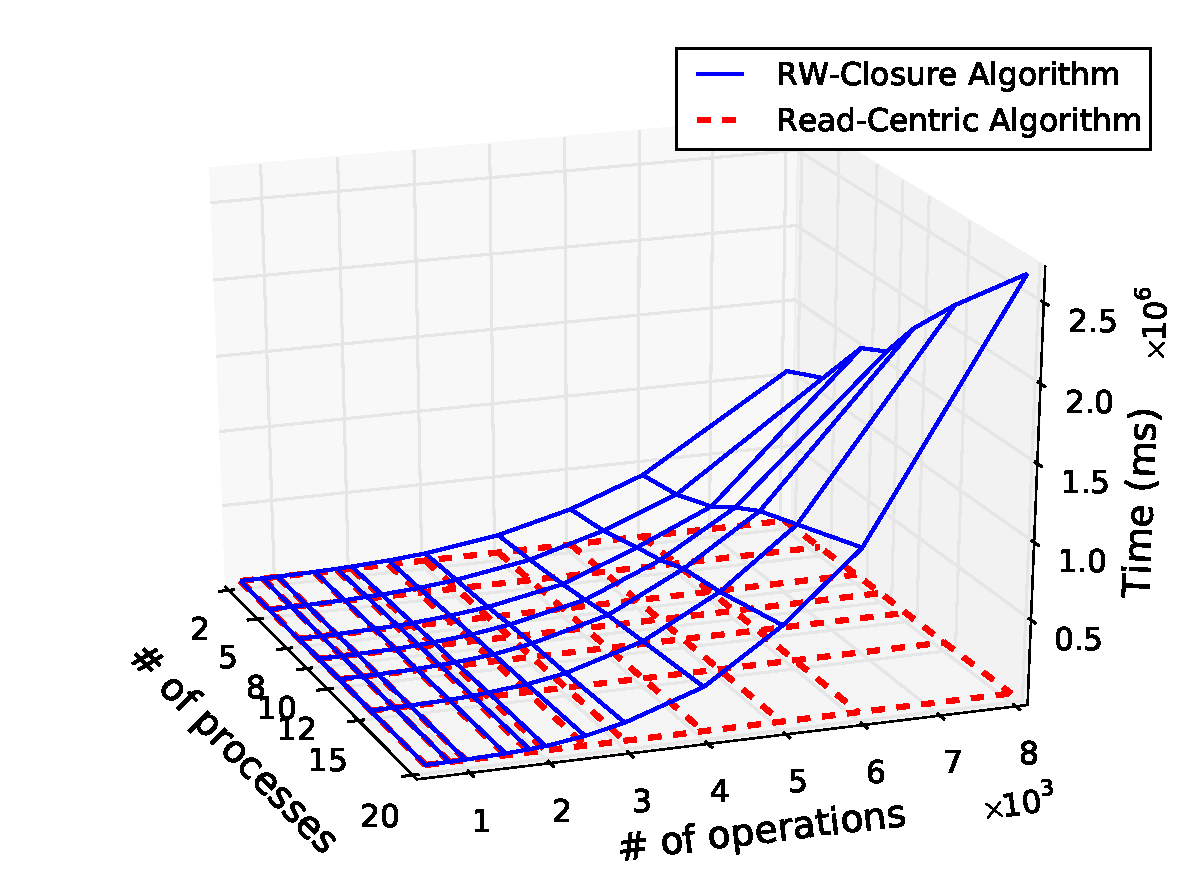
\includegraphics[width = 0.80\textwidth]{figures/vpc-valid-cmp.pdf}
	\end{subfigure}
	\caption{\rwclosure{} 算法与 \readcentric{} 算法在
	\textcolor{blue!80}{ (左) 随机生成}的执行及
	\textcolor{red!80}{ (右) 满足 \PRAM{} 一致性}的执行上的运行时间。}
  \end{figure}

  \pause
  \begin{center}
	\textcolor{red}{(右)} 20个进程、8,000 个操作: 

	\readcentric{} 可获得 694 倍加速.
  \end{center}
\end{frame}
%%%%%%%%%%%%%%%
\begin{frame}{实验评估}
  \fig{width = 0.50\textwidth}{figures/vpc-scalability-more.pdf}
  {\readcentric{} 算法在满足 \PRAM{} 一致性的执行上的运行时间.}

  \begin{description}
	\centering
	\item[\readcentric{}:] 20个进程、60,000个操作 < 600s
	\item[\rwclosure{}:] 20个进程、8,000个操作 > 3,000s
  \end{description}
\end{frame}
%%%%%%%%%%%%%%%
\begin{frame}{VPC 的意义}
  \mdf{red}{blue}{对 VPC 问题的系统研究}{teal}{
	\begin{enumerate}
	  \item \readcentric{} 算法可用于测试系统是否正确实现了 \PRAM{} 一致性模型
	  \item \npcn{} 结果有助于理解弱一致性模型的复杂度
	\end{enumerate}
  }
\end{frame}
%%%%%%%%%%%%%%%

%%%%%%%%%%%%%%%%%%%%%%%%%%%%%%%%%%%%%%%%	
\subsection{PA2AM: (2-)Atomicity 一致性维护与量化}

%%%%%%%%%%%%%%%
\begin{frame}{PA2AM 工作在技术框架中的位置}
  \fig{width = 0.50\textwidth}{figures/3d-framework-pa2am.pdf}{PA2AM --- (2-)Atomicity 一致性维护与量化.}
\end{frame}
%%%%%%%%%%%%%%%
\begin{frame}{研究动机}
  \question{问题: 为什么提出 probabilistically-atomic 2-atomicity {\small (PA2AM)} 一致性?}
  \vspace{0.30cm}

  \pause
  ``数据一致性/访问延迟'' PACELC 权衡 \citeinbeamer{Abadi}{IEEE Computer}{12}:

  \fignocaption{width = 0.35\textwidth}{figures/stronger-consistency-tradeoff.pdf}

  % \begin{quote}
  %   ``As soon as a distributed storage system replicates data, a \textcolor{brown}{tradeoff 
  %   between consistency and latency} arises.''
  % \end{quote}

  \pause

  ``低延迟''至关重要:
  \begin{itemize}
	\item 100ms 额外延迟 $\Rightarrow$ 1\% 销售下滑 \citeinbeamer{Amazon}{Blog}{06}
	\item 100$\sim$400ms 额外延迟 $\Rightarrow$ 0.2\%$\sim$0.6\% 搜索量下降 \citeinbeamer{Google}{Blog}{09}
  \end{itemize}

  % {\small
  % \begin{table}
  %   \begin{tabular}{c|c}
  %     \textcolor{blue}{\bf 系统} & \textcolor{blue}{\bf 一致性}		\\ \hline
  %     Dynamo@Amazon \citeinbeamer{Amazon}{SOSP}{07} & eventual consistency \\ \hline
  %     PNUTS@Yahoo! \citeinbeamer{Yahoo!}{PVLDB}{08} & cache consistency \\ \hline
  %     Tao@Facebook \citeinbeamer{Facebook}{ATC}{13} & $\le$ read-after-write \\ \hline
  %   \end{tabular}
  % \end{table}
  % }
\end{frame}
%%%%%%%%%%%%%%%
\begin{frame}{PA2AM 一致性}
  % \begin{cdef}[``近乎强''一致性]
  %   对某特定强一致性的弱化: \begin{itemize}
  %     \item (版本) 允许读陈旧值,但陈旧度有限
  %     \item (概率) 读到陈旧值的概率很小
  %   \end{itemize}
  % \end{cdef}

  \begin{center}
	\only<2->{\textcolor{blue}{``近乎强''一致性: }}{在保证\textcolor{red}{低延迟}的情况下获得\textcolor{red}{尽可能强}的数据一致性.}
  \end{center}

  \uncover<3->{
  \begin{cdef}[PA2AM 一致性]
	\begin{description}
	  \setlength{\itemsep}{5pt}
	  \item[低延迟:] \uncover<4->{读操作只需一轮网络通信} 
	  \item[尽可能强:] \uncover<6->{对 atomicity {\small (strongest)} 的弱化}
    \begin{itemize}
	  \item<6-> \textcolor{brown}{\it (版本)} 2-atomicity: 允许读陈旧值, 但\textcolor{red}{陈旧度 $k \le 2$}
	  \item<6-> \textcolor{brown}{\it (概率)} \textcolor{red}{$\mathbb{P}(k = 2)$ 很小}
    \end{itemize}
    \end{description}
  \end{cdef}
  }

  \vspace{0.20cm}
  \uncover<5->{
  \begin{ctheorem}[不可能性结果]
    (单写模型下) 不存在低延迟的 atomicity 维护算法 \citeinbeamer{Dutta}{PODC}{04}.
  \end{ctheorem}
  }
\end{frame}
%%%%%%%%%%%%%%%
\begin{frame}{PA2AM 维护算法}
  \fig{width = 0.80\textwidth}{figures/atomicity-2am-read-compare.pdf}
  {经典 atomicity 算法中, 读操作需两轮网络通信 \citeinbeamer{Attiya}{JACM}{95} 
  \citeinbeamer{Dutta}{PODC}{04}. 
  PA2AM 算法实现 2-atomicity {\scriptsize (单写模型下)}, 读操作只需一轮网络通信.}
\end{frame}
%%%%%%%%%%%%%%%
\begin{frame}{PA2AM 量化分析}
  \question{问题: PA2AM 算法在多大程度上违反了 atomicity?}
  \vspace{0.10cm}

  \begin{itemize}
    \setlength{\itemsep}{10pt}
	\item 充要条件: ONI (old-new inversion) \citeinbeamer{Attiya}{JACM}{95}
      \fignocaption{width = 0.45\textwidth}{figures/2atomicity-case.pdf}
    \item PA2AM 量化分析: 计算 $\mathbb{P}(\textrm{ONI})$, 其值越小越好
      \begin{enumerate}
        \setlength{\itemsep}{3pt}
        \item $\textrm{ONI} \triangleq \textrm{CP} \cap \textrm{RWP}$
        \item 排队论建模, 计算 $\mathbb{P}(\textrm{CP})$ \item 带时间的球盒模型, 计算 
          $\mathbb{P}(\textrm{RWP|CP})$
        % \item 实验统计 $\mathbb{P}(\textrm{CP})$, $\mathbb{P}(\textrm{RWP|CP})$ 与 
        % $\mathbb{P}(\textrm{ONI})$, 以作对照
      \end{enumerate}
  \end{itemize}
\end{frame}
%%%%%%%%%%%%%%%
\begin{frame}{PA2AM 量化分析}
  公式推导:
  \begin{figure}
	\begin{subfigure}{0.50\textwidth}
	  \centering
	  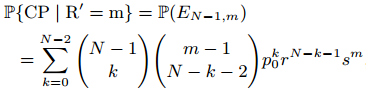
\includegraphics[width = 0.70\textwidth]{figures/cp.png}
	\end{subfigure}%
	\begin{subfigure}{0.50\textwidth}
	  \centering
	  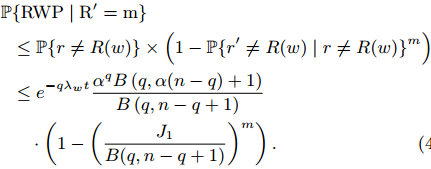
\includegraphics[width = 0.70\textwidth]{figures/rwp.png}
	\end{subfigure}
  \end{figure}

  \vspace{0.10cm}

  数值结果 (左一) 与实验结果 (右二): 
  \begin{figure}
	\begin{subfigure}{0.45\textwidth}
	  \centering
	  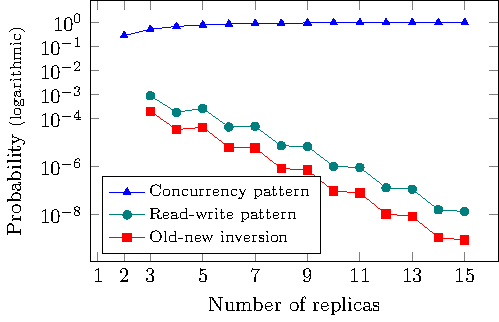
\includegraphics[width = 0.60\textwidth]{figures/oni-pgfplot.pdf}
	\end{subfigure}%
	\begin{subfigure}{0.55\textwidth}
	  \centering
	  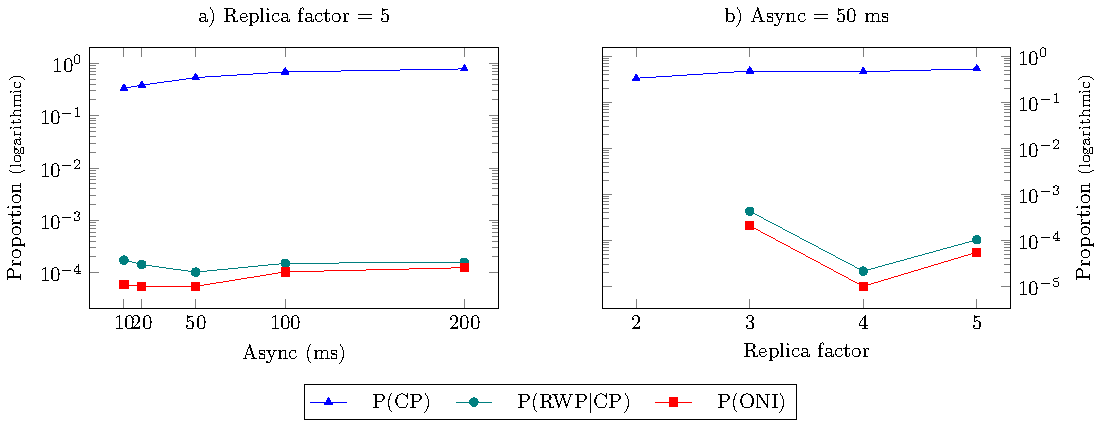
\includegraphics[width = 0.90\textwidth]{figures/experiment-oni-pgfplot.pdf}
	\end{subfigure}
  \end{figure}
\end{frame}
%%%%%%%%%%%%%%%
\begin{frame}{PA2AM vs. 弱一致性模型}
  \begin{figure}
	\begin{subfigure}{0.50\textwidth}
	  \centering
	  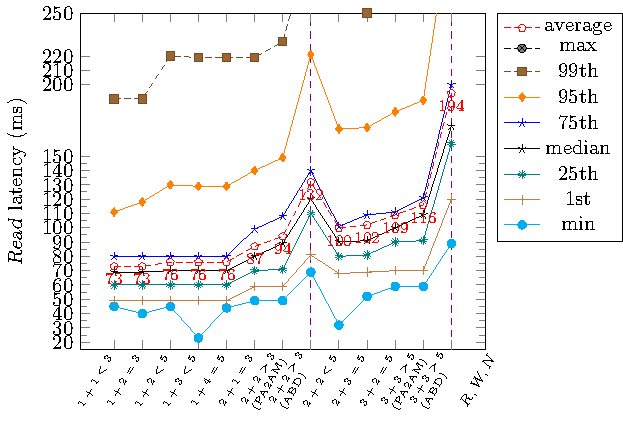
\includegraphics[width = 0.85\textwidth]{figures/rwn-2am-read-latency-quantiles.pdf}
	  \caption{读操作延迟对比.}
	\end{subfigure}%
	\begin{subfigure}{0.50\textwidth}
	  \centering
	  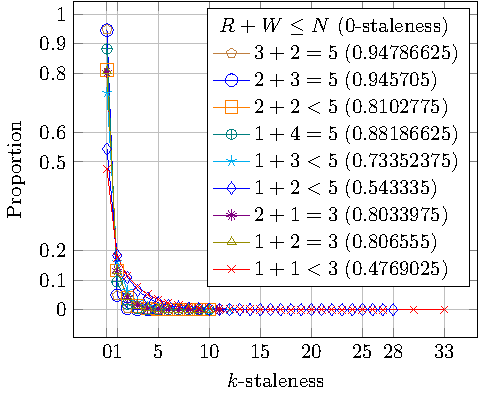
\includegraphics[width = 0.70\textwidth]{figures/rwn-maj.pdf}
	  \caption{$k$-陈旧度对比.}
	\end{subfigure}
	\caption{PA2AM 与 eventual consistency (RWN-Maj 协议) 对比结果.}
  \end{figure}

  \vspace{-0.50cm}
  \begin{table}[]
  \renewcommand{\arraystretch}{1.3}
  \centering
  \caption{不同 $R,W,N$ 配置下, RWN-All 执行中具有不同陈旧度的读操作的比率.}
  \label{tbl:rwn-all-staleness}
  \resizebox{\textwidth}{!}{%
  \begin{tabular}{|c||c|c|c|c||c|c|c|c|c|c|c|}
  \hline
  {\bfseries \# replicas} & \multicolumn{4}{c||}{\bfseries replica factor = 3 ($400,000$
    \textsl{read} operations)} & \multicolumn{7}{c|}{\bfseries replica factor = 5 ($800,000$
    \textsl{read} operations)} 
  \\ \hline
  {\bfseries $R,W,N$} % \textrm{R}+\textrm{W} $\boldsymbol{\le}$ \textrm{N}}  
  & $1+1<3$	& $1+2=3$	& $2+1=3$	& $2+2>3 \;(\text{PA2AM})$ 
  & $1+2<5$ 	& $1+3<5$ 	& $1+4=5$	& $2+2<5$ 	& $2+3=5$    & $3+2=5$     & $3+3>5 \;(\text{PA2AM})$     
  \\ \hline \hline
  {\boldmath $\max k$}          & $6$      & $4$ 	& $2$    &  {\boldmath $1$}
  & $2$	& $2$      	& $2$	   & $2$	& $2$	 &  $2$     & {\boldmath $1$}
  \\ \hline
  {\bfseries $\sum_{k \ge 1}$-staleness}       & $0.0084125$      & $0.000315$ 	&  $0.0004675$	&
  {\boldmath $0.000085$}
  	&  $0.00377875$	&  $0.002755$	&  $0.00406$     & $0.0027225$      & $0.0020275$     & $0.002255$      
	&  {\boldmath $0.0003525$}
  \\ \hline
  \end{tabular}%
}
\end{table}

\end{frame}
%%%%%%%%%%%%%%%
\begin{frame}{PA2AM 的意义}
  \mdf{red}{blue}{PA2AM 可作为一致性/延迟权衡的一种有价值的选项}{teal}{
	\begin{itemize}
	  \item 既 {\small (在统计意义上)} 满足强一致性模型对数据一致性的高标准
	  \item 又具有弱一致性模型的性能优势
    \end{itemize}
  }
\end{frame}
%%%%%%%%%%%%%%%

%%%%%%%%%%%%%%%%%%%%%%%%%%%%%%%%%%%%%%%%	
\subsection{RVSI: Snapshot Isolation 一致性弱化与维护}

\newcommand{\chameleon}{\textsc{Chameleon}}
\newcommand{\konebv}{$k_1$-BV}
\newcommand{\ktwofv}{$k_2$-FV}
\newcommand{\kthreesv}{$k_3$-SV}
%%%%%%%%%%%%%%%
\begin{frame}{RVSI 工作在技术框架中的位置}
  \fig{width = 0.50\textwidth}{figures/3d-framework-rvsi.pdf}
	{RVSI --- Snapshot Isolation 一致性弱化与维护.}
\end{frame}
%%%%%%%%%%%%%%%
\begin{frame}{研究动机}
  \question{问题: 为什么要提出 Relaxed Version Snapshot Isolation {\small (RVSI)} 一致性?}
  \vspace{0.20cm}

  \begin{description}
    \setlength{\itemsep}{5pt}
    \item[分布式事务:]
      \begin{itemize}
        \item ``all-or-none'' 语义
        \item 受到分布式存储系统的关注 \citeinbeamer{Cassandra}{CASSANDRA-ISSUE-7056}{14}
      \end{itemize}
    \item[弱一致性:] 
        PCSI \citeinbeamer{Elnikety}{SRDS}{05} 
		  \textcolor{red}{SI} \citeinbeamer{Lin}{TODS}{09} \\
          PSI \citeinbeamer{Sovran}{SOSP}{11} NMSI \citeinbeamer{Ardekani}{SRDS}{13} 
    \pause
	\item[\textcolor{red}{异常控制:}] 容忍``有限度的''异常 \citeinbeamer{Yu}{TOCS}{02}
	\item[\textcolor{red}{可调节:}] 
      \begin{itemize}
        \item 不同应用对一致性需求不同 \citeinbeamer{Terry}{CACM}{13}
        \item 运行时决定 \citeinbeamer{Terry}{SOSP\&TR}{13}
      \end{itemize}
  \end{description}
\end{frame}
%%%%%%%%%%%%%%%
\begin{frame}{RVSI 定义}
  RVSI 定义原则:
  \begin{itemize}
    \item 参数 $k_1, k_2, k_3$ 控制``异常''程度
    \item $\text{RC} \supset \text{RVSI}(k_1, k_2, k_3) \supset \text{SI}$
    \item $\text{RVSI}(\infty,\infty,\infty) = \text{RC}; \qquad \text{RVSI}(1,0,\ast) = \text{SI}$
  \end{itemize}

  \vspace{0.20cm}

  \begin{cdef}[RVSI: Relaxed Version Snapshot Isolation]
    \begin{description}
      \item[单变量读 $\texttt{read}(x)$:] \hfill 
        \begin{enumerate}
		  \item 允许读 $\le k_1$ 陈旧值 (\konebv{})
		  \item 允许读 $\le k_2$ 并发更新 (\ktwofv{})
        \end{enumerate}
      \item[多变量读 $\texttt{read}(x), \texttt{read}{(y)}$:] \hfill
        \begin{enumerate}
          \setcounter{enumi}{2}
		\item $\text{distance}(\textsl{snap}{(x)},\textsl{snap}{(y)}) \le k_3$
        \end{enumerate}
    \end{description}
  \end{cdef}
\end{frame}
%%%%%%%%%%%%%%%
\begin{frame}{\chameleon{} 分布式事务键值存储原型系统设计}
  \begin{description}
	\item[系统架构:] 阿里云\footnote{阿里云: \url{https://www.aliyun.com/}.} 
	  多数据中心 {\small ($9 = 3 \times 3$)}
	\item<2->[数据分区:] 同一数据中心
	\item<2->[数据副本:] 跨数据中心; 主从结构
  \end{description}

  \fignocaption{width = 0.55\textwidth}{figures/chameleon-arch.pdf}
\end{frame}
%%%%%%%%%%%%%%%
\begin{frame}{\chameleon{} 分布式事务键值存储原型系统设计}
  \begin{description}
	\item[系统组件:] 客户端库 + 数据中心
	\item<2->[数据分区:] 分布式事务原子提交协议 {\small (2PC)}
	\item<2->[数据副本:] 懒惰复制 {\small (lazy replication)} 协议
  \end{description}

  \fignocaption{width = 0.42\textwidth}{figures/chameleon-framework.pdf}
\end{frame}
%%%%%%%%%%%%%%%
\begin{frame}{RVSI 维护算法}
  \[
    \textcolor{blue}{\text{RC} \supset \text{RVSI}(k_1, k_2, k_3) \supset \text{SI}}
  \]

  \vspace{0.10cm}

  RVSI 维护算法:
  \begin{itemize}
    \item 以分布式 RC 和 SI 协议 为基础
    \item 事务执行时, 添加 RVSI ``版本约束'' ($k_1, k_2, k_3$ 相关不等式)
    \item 事务提交时, 检查 RVSI ``版本约束''
  \end{itemize}

  % \fignocaption{width = 0.50\textwidth}{figures/chameleon-build-passing.png}
  \textcolor{red}{\small \url{https://github.com/hengxin/chameleon-transactional-kvstore}}
\end{frame}
%%%%%%%%%%%%%%%
\begin{frame}{RVSI 实验评估}
  \begin{table}[]
  \renewcommand{\arraystretch}{1.1}
  \centering
  \caption{事务负载参数表.\protected\\(\textcolor{blue}
	{评估目标: RVSI 对事务中止率的影响})}
  \resizebox{\textwidth}{!}{%
  \begin{tabular}{|c||c|c|c|}
	\hline
	{\bfseries Parameter}   & {\bfseries F(ixed)/V(ariable)/R(andom)}	
	& {\bfseries Value}		& {\bfseries Explanation}
	\\ \hline  \hline
	\#keys  				& F		& 5  				&  	size of keyspace
	\\ \hline
	\cellcolor{brown}mpl	& \textcolor{red}{\bf V}		& 5, 10, 15, 20, 25, 30
	& \innercell{c}{multiprogramming level: \\ number of concurrent clients} \\ \hline
	\#txs/client					& F		& 1000 						
	& \innercell{c}{number of txs per client}
	\\ \hline
	\#ops/tx					& R		& $\sim$ Binomial(20, 0.5)	
	&  \innercell{c}{number of operations per tx}
	\\ \hline
	\cellcolor{brown}rwRatio & \textcolor{red}{\bf V} 
	  & 1:2, 1:1, 4:1 & {\#reads}/{\#writes}
	\\ \hline
	zipfExponent			& F		& 1		& parameter for Zipfian distribution
	\\ \hline  \hline
	\cellcolor{brown}$(k_1, k_2, k_3)$		& \textcolor{red}{\bf V}
		&  \innercell{c}{(1,0,0) \\ (1,0,2) (1,1,0) \\ (2,0,0) (2,1,2) (2,2,1)}	
		&  for \konebv{}, \ktwofv{}, and \kthreesv{}
	\\ \hline  \hline
	minInterval				& F		& 0ms		& minimum inter-transactions time
	\\ \hline
	maxInterval				& F		& 10ms		& maximum inter-transactions time
	\\ \hline
	meanInterval			& R		& 5ms		
	& \innercell{c}{mean inter-transactions time \\ for exponential distribution}
	\\ \hline
  \end{tabular}
  }
\end{table}

\end{frame}
%%%%%%%%%%%%%%%
\begin{frame}{RVSI 实验评估}
  \fig{width = 0.70\textwidth}{figures/rvsi-rw4-abort-rates.pdf}
	{读频繁 (rwRatio = 4:1) 负载下 RVSI 对事务中止率的影响.}

  \begin{description}
	\item[\textcolor{blue}{wcf-aborted:}] 
	  无显著变化 {\small ($\text{wcf}(1,0,0) = 0.184733$)}
	\item[\textcolor{red}{vc-aborted:}] 显著减少 
	  {\small ($\text{vc}(1,0,0) = 0.204733;
	  \text{vc}(1,1,0) = 0.066433;
	  \text{vc}(2,2,1) = 0.002033$)}
  \end{description}
\end{frame}
%%%%%%%%%%%%%%%
\begin{frame}{RVSI 实验评估}
  \begin{columns}
	\column{0.48\textwidth}
	  \fig{width = 1.00\textwidth}{figures/rvsi-rw05-abort-rates.pdf}
		{写频繁 (rwRatio = 1:2) 负载下 RVSI 对事务中止率的影响.}
	\column{0.48\textwidth}
	  \fig{width = 1.00\textwidth}{figures/rvsi-rw1-abort-rates.pdf}
		{读写相当 (rwRatio = 1:1) 负载下 RVSI 对事务中止率的影响.}
  \end{columns}
\end{frame}
%%%%%%%%%%%%%%%
\begin{frame}{RVSI 的意义}
  \mdf{red}{blue}{RVSI 对事务中止率的影响}{teal}{
	\begin{enumerate}
	  \item 适当放松事务对 RVSI 版本规约的要求可降低事务中止率
	  \item RVSI 能否``显著''降低事务中止率与负载类型相关
    \end{enumerate}
  }
\end{frame}
%%%%%%%%%%%%%%%

%%%%%%%%%%%%%%%
